\documentclass[aps,onecolumn,12pt]{revtex4}
\usepackage{graphicx}
\usepackage{amssymb,amsfonts,amsmath,amsthm}
\usepackage{chemarr}
\usepackage{bm}
\usepackage{pslatex}
\usepackage{xfrac}
\usepackage[dvipsnames]{xcolor}
%\usepackage{bookman}
\usepackage{dsfont}
\usepackage{mathptmx}
\usepackage{hyperref}
%\usepackage{rotating}

%%%%%%%%%%%%%%%%%%%%%%%%%%%%%%%%%%%%%%%%%%%%%%%%%%%%%%%%%%%%%%%%%%%%%%%%%%%%%%
%%
%%
%% Style
%%
%%
%%%%%%%%%%%%%%%%%%%%%%%%%%%%%%%%%%%%%%%%%%%%%%%%%%%%%%%%%%%%%%%%%%%%%%%%%%%%%%
\newcommand{\mychem}[1]{\mathtt{#1}}
\newcommand{\myconc}[1]{\left\lbrack{#1}\right\rbrack}

\newcommand{\spLi}[1]{{~^{\mychem{#1}}\mychem{Li}}}
\newcommand{\Li}[1]{\myconc{\spLi{#1}}}

\newcommand{\spEout}{\mychem{E}}
\newcommand{\Eout}{\myconc{\spEout}}

%\newcommand{\spLiEin}[1]{\left\lbrace\spLi{#1}\spEout\right\rbrace_{\mathrm{in}}}
%\newcommand{\LiEin}[1]{\myconc{\spLiEin{#1}}}

\newcommand{\spLiE}[1]{\left\lbrace\spLi{#1}\spEout\right\rbrace}
\newcommand{\LiE}[1]{\myconc{\spLiE{#1}}}


%\newcommand{\spLiEout}[1]{\left\lbrace\spLi{#1}\spEout\right\rbrace_{\mathrm{out}}}
%\newcommand{\LiEout}[1]{\myconc{\spLiEout{#1}}}

\newcommand{\spLiIn}[1]{{\spLi{#1}}_{\mathrm{in}}}
\newcommand{\LiIn}[1]{\myconc{\spLiIn{#1}}}

\newcommand{\spLiOut}[1]{{\spLi{#1}}_{\mathrm{out}}}
\newcommand{\LiOut}[1]{\myconc{\spLiOut{#1}}}

\newcommand{\spEHin}{\mychem{EH}}
\newcommand{\EHin}{\myconc{\spEHin}}
\newcommand{\spproton}{\mychem{H}}
\newcommand{\proton}{\myconc{\spproton}}

\newcommand{\mytrn}[1]{{#1}^{\!\mathsf{T}}}
\newcommand{\mymat}[1]{{\bm{#1}}}
\newcommand{\mydet}[1]{{\left|{#1}\right|}}

\newcommand{\ratioLi}{ {\left(\dfrac{\Li{7}}{\Li{6}}\right)} }
\newcommand{\deltaLi}{ {\delta\!\!\!\spLi{7}} }
\newcommand{\deltaLiOut}{{\deltaLi}_{\mathrm{out}}}

\newcommand{\LiAll}{\Lambda}
\newcommand{\LiAllOut}{{\LiAll}_{\mathrm{out}}}

\newcommand{\NHE}[1]{\mychem{NHE}{\mychem{\hbox{-}\!#1}}}
\newcommand{\todo}[1]{\framebox{\textbf{\color{WildStrawberry}{#1}}}}

\newcommand{\ko}{\dagger}
\newcommand{\start}{\ast}

\DeclareMathOperator\erf{erf}
\newcommand{\pH}{\ensuremath{\mathrm{pH}}}

%%%%%%%%%%%%%%%%%%%%%%%%%%%%%%%%%%%%%%%%%%%%%%%%%%%%%%%%%%%%%%%%%%%%%%%%%%%%%%
%%
%%
%% Document
%%
%%
%%%%%%%%%%%%%%%%%%%%%%%%%%%%%%%%%%%%%%%%%%%%%%%%%%%%%%%%%%%%%%%%%%%%%%%%%%%%%%


\begin{document}
\title{Supplementary Material...}
\maketitle

\section{Setting up the Model}

\subsection{Description And Notations}

\subsubsection{Isotopic Ratio}
The isotopic separation of a mixture of $\spLi{6}$ and $\spLi{7}$ is defined by:
\begin{equation}
	\deltaLi = \left(
		\dfrac{\left(\dfrac{\Li{7}}{\Li{6}}\right)_{sample}}
		{\left(\dfrac{\Li{7}}{\Li{6}}\right)_{standard}}
		 -1 
	\right) \times 1000,
\end{equation}
or
\begin{equation}
	\left(\dfrac{\Li{7}}{\Li{6}}\right)_{sample} = \left(\dfrac{\Li{7}}{\Li{6}}\right)_{standard} \left[1+10^{-3}\deltaLi\right] = \lambda_s \left[1+10^{-3}\deltaLi\right].
\end{equation}
We define
\begin{equation}
\left\lbrace
\begin{array}{rclcl}
	\LiAll & = & \Li{6} + \Li{7}\\
	\Li{6} & = & \dfrac{1}{1+\lambda_s \left[1+10^{-3}\deltaLiOut\right] } \LiAllOut & = & \epsilon_6 \LiAllOut   \\
	\\
	\Li{7} & = & \dfrac{\lambda_s \left[1+10^{-3}\deltaLiOut\right]}{1+\lambda_s \left[1+10^{-3}\deltaLiOut\right] } \LiAllOut & = & \epsilon_7 \LiAllOut\\
\end{array}
\right.
\end{equation}

For the presented experiments, the lithium composition is:
\begin{equation}
	\lambda_s = 12.0192, \; \deltaLi = 14.57 \Rightarrow \epsilon_6 \simeq 0.076,\;\epsilon_7 \simeq 0.924
\end{equation}


\subsubsection{Lithium Transport}

Let us describe how a cell may intake a lithium isotope from the outer medium, which is formally described by the transformation
of $\spLiOut{x}$ into $\spLi{x}$ for $x=\lbrace 6,7 \rbrace$. We distinguish two main paths.

\begin{itemize}
\item We assume that the Enzymatic Path, using $\NHE{1}$ as the enzyme $\spEout$ works as follows. A more detailed description is found in \todo{ref}.
	\begin{itemize}
	\item The outer lithium is associated with a membrane enzyme:
	\begin{equation}
		\label{eq:pre}
		\spLiOut{x} + \spEout  \xrightleftharpoons[~~k^d_x~~]{~~k^a_x~~} \spLiE{x},
	\end{equation}
	where $k^a_x$ and $k^d_x$ respectively are the association and the dissociation rate constants.
	
	\item Then the associated complex exchange an inner proton with a lithium ion:
	\begin{equation}
		\label{eq:xch}
		\spLiE{x} + \spproton   \xrightleftharpoons[~~q_x~~]{~~k^p_x~~}   \spEHin + \spLi{x}, 
	\end{equation}
	where $k^p_x$ and $k^q_x$ respectively are the forward and reverse protonation rate constants.
	
	\item The attached inner proton is then transported out of the cell to recycle the enzyme:
	\begin{equation}
			\spEHin   \xrightarrow{~~k_h~~}   \spEout + \spproton_{\mathrm{out}} 
	\end{equation}	
	where $k_h$ is the  apparent recycling constant rate, assuming that $\spEHin$ is the predominant form of the enzyme at the inner membrane surface \todo{Lacroix EMBO 2004 fig 3A}.
	\end{itemize}

\item The Passive Path (or Leak) consists in the use by the lithium species of some ion channels, following the electro-osmotic gradient as described by the Goldman-Hodkins-Katz \todo{ref} equations and leading to:
	\begin{equation}
	\label{eq:ghk}
		\spLiOut{x} \xrightleftharpoons[~~k_x~~]{~~k_x e^{-\frac{FV_m}{RT}}~~}   \spLi{x} 
	\end{equation}
where $V_m$ is the membrane potential, $F$ is the Faraday's constant, $R$ is the perfect gas constant, and $T$ is the absolute temperature.

\end{itemize}

\subsubsection{Internal Proton Concentration}
Even if we account here the proton as a transported species, it is also a reactive species which is involved in many reactions, as to ensure the cell homeostasis\todo{ref}. That is why we consider $\proton$ as a heuristic function of time, which will very depend on the full cell pH regulation process.

\subsubsection{Membrane Potential Regulation}
The full system is electroneutral, since it globally exchanges one $\spproton$ per one $\spLi{x}$. Though the Nernst's potential and currents are likely to be displaced \todo{more explanations?}

\subsection{Full Kinetic Scheme}
We define the 11 following rates:
\begin{equation}
	\label{eq:rates}
\left\lbrace
\begin{array}{rcl}
	v^a_x & = & k^a_x \Eout \LiOut{x} \\
	\\
	v^d_x & = & k^d_x \LiE{x} \\
	\\
	v^p_x & = & k^p_x \LiE{x} \proton\\
	\\
	v^q_x & = & q_x \Li{x} \EHin\\
	\\
	v_h   & = & k_x \EHin\\
	\\
	v^l_x & = & k_x\left(\Theta \LiOut{x} - \Li{x}\right),\;\;\Theta = e^{-\frac{FV_m}{RT}}\\
\end{array}
\right.
\end{equation}
We deduce the full constrained kinetic scheme with 6 variables:
\begin{equation}
	\label{eq:full}
\left\lbrace
\begin{array}{rcl}
\partial_t \EHin & = & -v_h + \sum_x\left(v^p_x - v^q_x\right)\\
\\
\partial_t \Eout & = & v_h + \sum_x(v^a_x -v^d_x)\\
\\
\partial_t \LiE{x} & = & v^a_x -v^d_x + v^q_x -v^p_x\\
\\
\partial_t \Li{x}  & = & v^l_x + v^p_x - v^q_x\\
\end{array}
\right.
\end{equation}
and we check that we always verify the conservation:
\begin{equation}
	E_0  =  \Eout + \EHin + \LiE{6} + \LiE{7},
\end{equation}
where $E_0$ is the cellular total $\NHE{1}$ membrane concentration.

\subsection{Complexity Reduction by Semi-Stationary Kinetic Scheme}

\subsubsection{Algebraic Simplification}
We assume that the binding of the outer lithium to the enzyme is fast compared to its subsequent transport through the membrane. 
Accordingly, we define the two equilibria:
\begin{equation}
\label{eq:J}
\spLiOut{x} +  \spEout    \xrightleftharpoons[]{}  \spLiE{x}, \;\; J_x = \dfrac{\LiE{x}}{\LiOut{x} \Eout} = \dfrac{k_x^a}{k_x^d},
\end{equation}
which shall be always verified.
We now harness the algebraic method previously established\todo{ref} to end up with only 3 coupled equations:
\begin{equation}
\label{eq:sys}
\left\lbrace
	\begin{array}{rcl}
		\partial_t\EHin & = & -k_h \EHin + \left(E_0- \EHin\right) \dfrac{\proton}{\mathfrak{D}} \left(\sum_x k_x^p J_x\LiOut{x} \right)  
		- \EHin \left({\sum_x q_x \Li{x}} \right)
		\\
		\\
		& = & 
		-k_h E_0+ \left(E_0- \EHin\right)\left\lbrack k_h+ \dfrac{\proton}{\mathfrak{D}} \left(\sum_x k_x^p J_x\LiOut{x}\right)\right] 
		- \EHin \left( {\sum_x q_x \Li{x}} \right)
		\\
		\\
		\partial_t\Li{x} & = & k_x \left(\Theta\LiOut{x} -\Li{x} \right)  + \left(E_0-\EHin\right) \dfrac{\proton}{\mathfrak{D}}   k_x^p  J_x \LiOut{x}  
		- \EHin q_x \Li{x}
		\\
		\\
		(\mathfrak{D} & = & 1+\sum_x J_x \LiOut{x} )\\
	\end{array}
\right.
\end{equation}

\subsubsection{Rescaling and rewriting}
We define the following set of variables:
\begin{equation}
\label{eq:scale}
\left\lbrace
\begin{array}{rcll}
	\alpha & = & \dfrac{\EHin}{E_0} & \text{(fraction of protonated enzyme)}\\
	\\
	\hat\alpha & = & 1-\alpha       & \text{(fraction of not protonated enzyme)}\\
	\\
	\beta_x    & = & \dfrac{\Li{x}}{\LiOut{x}} & \text{(internal lithium amplification factor)}\\
	\\
	J_\epsilon & = & \sum_x \epsilon_x J_x & \text{(mixed affinity)}\\
	\\
	\LiAllOut  & = & \LiOut{6} + \LiOut{7} & \text{(external lithium concentration)}\\
\end{array}
\right..
\end{equation}
Then we rewrite:
\begin{equation}
\label{eq:sysnew}
\left\lbrace
\begin{array}{rcl}
	\partial_t \alpha & = & -k_h \alpha + \LiAllOut \left[ (1-\alpha) \proton  \dfrac{ \left(\sum_x k^p_x \epsilon_x J_x\right) }{1+J_\epsilon\LiAllOut}
	-\alpha  \left(\sum_x q_x \epsilon_x \beta_x \right)\right]
	\\
	\\
	\partial_t \beta_x & = & k_x\left(\Theta - \beta_x\right) +E_0\left[ (1-\alpha)  \proton \dfrac{k^p_x J_x}{1+J_\epsilon \LiAllOut} - \alpha q_x \beta_x \right]
\end{array}
\right.,
\end{equation}
or, in terms of $\hat\alpha$:
\begin{equation}
\label{eq:sysbis}
\left\lbrace
\begin{array}{rcl}
	\partial_t \hat\alpha & = & k_h  
		- \hat\alpha\left\lbrack k_h+ \proton  \dfrac{ \LiAllOut \left(\sum_x k^p_x \epsilon_x J_x\right) }{1+J_\epsilon\LiAllOut}\right] 
		+ (1-\hat\alpha) \LiAllOut\left( {\sum_x q_x \epsilon_x \beta_x} \right)
	\\
	\\
	\partial_t \beta_x & = & k_x\left(\Theta - \beta_x\right) +E_0\left[ \hat\alpha  \proton \dfrac{k^p_x J_x}{1+J_\epsilon \LiAllOut} - (1-\hat\alpha) q_x \beta_x \right]\\
\end{array}
\right.
\end{equation}
It is interesting to define:
\begin{equation}
\label{eq:upsilon}
\left\lbrace
\begin{array}{rcll}
	\Upsilon_x & = & \dfrac{k^p_x J_x}{1+J_\epsilon \LiAllOut} & \text{(with lithium dependent saturation effect)}\\
	\Upsilon_6 & = & \gamma \Upsilon_7 & \text{($\gamma$=intake speed up)} \\
	\Upsilon_\alpha & = & \epsilon_6 \Upsilon_6 + \epsilon_7 \Upsilon_7 = \underbrace{(\epsilon_6 \kappa + \epsilon_7)}_{\kappa'} \Upsilon_7 & 
	\text{(mixed intake coefficient)}\\
\end{array}
\right.
\end{equation}
and to formally write the coupled system:
\begin{equation}
\label{eq:sysall}
\left\lbrace
\begin{array}{rcl}
\partial_t \hat\alpha & = &
	 k_h \left(1-\hat\alpha\right) 
	 + \LiAllOut \left[ (1-\hat\alpha) \left( {\sum_x q_x \epsilon_x \beta_x} \right)  - \hat\alpha\proton \Upsilon_\alpha \right]\\
	 \\
\partial_t \alpha & = & -k_h \alpha + \LiAllOut \left[ (1-\alpha) \proton  \Upsilon_\alpha
	-\alpha  \left(\sum_x q_x \epsilon_x \beta_x \right)\right]\\
\\
	\partial_t \beta_x & = & k_x\left(\Theta - \beta_x\right) +E_0\left[ \hat\alpha  \proton \Upsilon_x - (1-\hat\alpha) q_x\beta_x \right]\\
	\\
	 & = & k_x\left(\Theta - \beta_x\right) +E_0\left[ (1-\alpha)  \proton \Upsilon_x - \alpha q_x \beta_x \right]
\end{array}
\right.
\end{equation}

The initial conditions for those equivalent systems are written as:
\begin{equation}
\label{eq:ini}
\left\lbrace
\begin{array}{rcl}
\alpha(t=0) & = & 0\\
\hat\alpha(t=0) &= & 1\\
\beta_x(t=0)    &=& 0\\
\end{array}
\right.
\end{equation}

The isotopic separation is related to the amplification factor by:
\begin{equation}
	r=\dfrac{ \beta_7}{\beta_6} = \dfrac{\left[1+10^{-3}\deltaLi\right]}{\left[1+10^{-3}\deltaLiOut\right]}
	.
\end{equation}

\subsection{Potential}
\begin{equation}
\left\lbrace
\begin{array}{rcll}
	\dfrac{FV_m}{RT} & \simeq & \dfrac{FV_0}{RT} + \zeta_m \LiAll & = \zeta_0 + \zeta_m \LiAll\\
	\\
	\Theta & = & \exp\left[ - \dfrac{FV_m}{RT}\right] & \simeq \Theta_0 e^{-u \left(\epsilon_6 \beta_6 + \epsilon_7 \beta_7 \right) }
	\\
\end{array}
\right.
\end{equation}
~\\
Let us assume that
\begin{equation}
	\partial_t \beta = k \left(\Theta-\beta\right) = k\left(\Theta_0e^{-u\beta} - \beta\right) \simeq k \left( \dfrac{\Theta_0}{1+u\beta} - \beta\right)
\end{equation}
we get
\begin{equation}
	\dfrac{1+u\beta}{u\beta^2+\beta-\Theta_0} \partial_t \beta = -k
\end{equation}
using
\begin{equation}
\left\lbrace
\begin{array}{rcl}
	\beta^{\pm} & = & \dfrac{-1\pm\sqrt{1+4u\Theta_0}}{2u}\\
	\\
	\beta^\infty & = & \beta^+  = \dfrac{\sqrt{1+4u\Theta_0}-1}{2u} \in [0:\Theta_0]\\
	\\
	\beta^\star & = & -\beta^- = \dfrac{\sqrt{1+4u\Theta_0}+1}{2u}\\
\end{array}
\right.
\end{equation}

we write
\begin{equation}
	\dfrac{1}{u\beta^2+\beta-\Theta_0} = \dfrac{1}{\sqrt{1+4u\Theta_0}}\left[\dfrac{1}{\beta-\beta^+}-\dfrac{1}{\beta-\beta^-}\right]
\end{equation}
so that
\begin{equation}
	\left(1+u\beta\right) \left[\dfrac{1}{\beta-\beta^+}-\dfrac{1}{\beta-\beta^-}\right] \partial_t \beta = - k \sqrt{1+4u\Theta_0}
\end{equation}
or
\begin{equation}
	 \left[ \dfrac{1+u\beta^+}{\beta-\beta^+} - \dfrac{1+u\beta^-}{\beta-\beta^-} \right] \partial_t \beta = - k \sqrt{1+4u\Theta_0}.
\end{equation}
We integrate
\begin{equation}
	\left(1+u\beta^+\right) \ln\left[ \dfrac{\beta^+-\beta}{\beta^+}\right] 
	- \left(1+u\beta^-\right) \ln\left[ \dfrac{\beta^--\beta}{\beta^-}\right] = -\left(k \sqrt{1+4u\Theta_0}\right) t 
\end{equation}
leading to
\begin{equation}
	\left(1+\sqrt{1+4u\Theta_0}\right) \ln\left[ \dfrac{\beta^\infty-\beta}{\beta^\infty}\right] 
	- \left(1-\sqrt{1+4u\Theta_0}\right) \ln\left[ \dfrac{\beta+\beta^\star }{\beta^\star}\right] = -\left(2 k \sqrt{1+4u\Theta_0}\right) t 
\end{equation}
or
\begin{equation}
	\ln\left[ \dfrac{\beta^\infty-\beta}{\beta^\infty}\right]
	 + \dfrac{4u\Theta_0}{\left[1+\sqrt{1+4u\Theta_0}\right]^2} \ln \left[ \dfrac{\beta+\beta^\star }{\beta^\star}\right] = - \dfrac{2 k \sqrt{1+4u\Theta_0}}{\left(1+\sqrt{1+4u\Theta_0}\right)} t
\end{equation}
Using
\begin{equation}
	Z_u =  \dfrac{4u\Theta_0}{\left[1+\sqrt{1+4u\Theta_0}\right]^2} \in \lbrack0:1\lbrack
\end{equation}
we obtain a compact form
\begin{equation}
	\ln\left[ \dfrac{\beta^\infty-\beta}{\beta^\infty}\right]
	 + Z_u \ln \left[ \dfrac{\beta+\beta^\star }{\beta^\star}\right] = -\left(1+Z_u\right) k t
\end{equation}
that becomes:
\begin{equation}
	\left[ \dfrac{\beta^\infty-\beta}{\beta^\infty}\right] \left[1+\dfrac{\beta}{\beta^\star}\right]^{Z_u}= e^{  -\left(1+Z_u\right) k t }
\end{equation}
Since $\beta\leq\Theta_0$, $1/\beta^\star\in[0,\sqrt{\frac{u}{\Theta_0}}]$, we assume
using 
\begin{equation}
	Y_u = \dfrac{Z_u}{\beta^\star} =  \dfrac{8u^2\Theta_0}{\left[1+\sqrt{1+4u\Theta_0}\right]^3}
\end{equation}
and noting that
\begin{equation}
	Y_u \beta^\infty = \dfrac{(4u\Theta_0)^2}{\left[1+\sqrt{1+4u\Theta_0}\right]^4} = Z_u^2 \in  \lbrack0:1\lbrack
\end{equation}

\begin{equation}
	Y_u \beta^2 + \left(1-Y_u\beta^\infty\right) \beta - \beta^\infty\left(1-e^{  -\left(1+Z_u\right) k t }\right) = 0
\end{equation}
\begin{equation}
\left\lbrace
\begin{array}{rcl}
	\beta & = & \dfrac{-\left(1-Y_u\beta^\infty\right) + \sqrt{ \left(1-Y_u\beta^\infty\right)^2 + 4Y_u\beta^\infty \left[1-e^{  -\left(1+Z_u\right) k t }\right]}}{2Y_u}\\
	\\
	& = & \beta^\infty \left( 
	\dfrac{
	\left(Z_u^2-1\right)
	+
	\sqrt{
		\left(Z_u^2-1\right)^2 + 4 Z_u ^2 \left[1-e^{  -\left(1+Z_u\right) k t }\right]
		}
	}
	{2Z_u^2}
	\right)
\end{array}
\right.
\end{equation}


\section{Boundary Values}

\subsection{Initial Times}

\begin{equation}
	\beta_x \simeq \left( k_x \Theta_0 + E_0 h_0 \Upsilon_x \right) t 
\end{equation}

\begin{equation}
	r_0 = \dfrac{k_7 \Theta_0 + E_0 h_0 \Upsilon_7}{k_6 \Theta + E_0 h_0 \Upsilon_6 }
\end{equation}

We define the amplification factor:
\begin{equation}
	\mu = \dfrac{E_0 h_0 \Upsilon_7}{k_7\Theta_0}
\end{equation}
so that:
\begin{equation}
	r_0 = \dfrac{1+\mu}{\sigma+\mu\gamma} \in \left[ \dfrac{1}{\gamma};\dfrac{1}{\sigma}\right].
\end{equation}
Since we have
\begin{equation}
	r_0 \leq \dfrac{1}{\sigma} \;\; \left(r_0\sigma \leq 1 \right).
\end{equation}
once we choose an amplification factor (that shall depends on $\LiAllOut$), then
the isotopic speedup $\gamma$ is:
\begin{equation}
	\gamma = \dfrac{1+\mu}{\mu}\left(\dfrac{1}{r_0} - \dfrac{\sigma}{1+\mu}\right)
\end{equation}

\subsection{Steady State}
\begin{equation}
	\alpha_\infty = \sin^2 \Omega, \hat\alpha_\infty = \cos^2 \Omega
\end{equation}

\begin{equation}
\begin{array}{rcl}
	\beta_x^\infty & = & \dfrac{k_x\Theta+E_0 h_\infty \Upsilon_x \cos^2\Omega}{k_x+E_0q_x\sin^2\Omega}\\
	\\
	\sin^2\Omega   & = & \dfrac{\LiAllOut h_\infty \Upsilon_\alpha}{k_h^\infty + \LiAllOut\left[ h_\infty \Upsilon_\alpha + \left(\sum_x q_x \epsilon_x \beta_x^\infty\right)\right]}\\
	\\
	\cos^2 \Omega  & = & \dfrac{k_h^\infty + \LiAllOut\left(\sum_x q_x \epsilon_x \beta_x^\infty\right) }{k_h^\infty + \LiAllOut\left[ h_\infty \Upsilon_\alpha + \left(\sum_x q_x \epsilon_x \beta_x^\infty\right)\right]}\\
\end{array}
\end{equation}





%%%%%%%%%%%%%%%%%%%%%%%%%%%%%%%%%%%%%%%%%%
\section{Information from Experiments}
\subsection{Information from Leakage}

\subsubsection{Passive Isotopic Separation}
With $E_0=0$, we readily obtain:
\begin{equation}
	\beta^\ko_x = \Theta \left(1-e^{-k_xt} \right),
\end{equation}
leading to the leak-only ratio:
\begin{equation}
	r^\ko(t) =  \dfrac{\left(1-e^{-k_7t} \right)}{\left(1-e^{-k_6t} \right)},\;r^\ko_0 = r^\ko(t\to0) = \dfrac{k_7}{k_6}.
\end{equation}
We define the \textit{passive isotopic ratio}:
\begin{equation}
\label{eq:sigma}
	\sigma  =  \dfrac{k_6}{k_7}.
\end{equation}
The GHK theory states that a diffusive-like behaviour is expected through the ion channels that lithium isotopes will cross.
We hence expect the ratio of the constant rates ($k_x$) to be in the same order of magnitude, so we assume \todo{ref}:
\begin{equation}
	\sigma \simeq 1.00229,
\end{equation}
and without active contribution, the initial isotopic ratio amounts to:
\begin{equation}
	r_0^\ko = \dfrac{1}{\sigma} \Rightarrow \deltaLi^\ko \simeq  12.25,
\end{equation}
which is far greater than the observed values even after some time \todo{ref figures in manuscript+values}


\subsubsection{Global Passive Lithium Intake}
Likewise, for membrane potential around $40\,\text{mV}$ at $37^\circ\text{C}$:
\begin{equation}
\label{eq:ThetaValue}
	\Theta = \exp\left( -\dfrac{FV_m}{RT}\right) \approx 4.47,
\end{equation}
which means that the amplification factor shall be greater than this value, and eventually the inner lithium concentration shall
be a few times the outer concentration. Indeed, the passive lithium intake is described by:
\begin{equation}
\label{eq:LiAllKO}
	\LiAll^\ko = \LiAllOut \Theta \left[ \epsilon_6 \left(1-e^{-k_6t}\right)  + \epsilon_7 \left(1-e^{-k_7t}\right)\right]
\end{equation}

The catalytic pathway can be simply discarded through two conditions:
\begin{itemize}
	\item we block $\NHE{1}$ by keeping the acidic medium,
	\item we use   $\mychem{PS120}$ cells which lack $\NHE{1}$
\end{itemize}
In both cases, we shall observe a slow lithium intake following Eq.\eqref{eq:LiAllKO}, which is fitted on figure \ref{fig:leak}.
\begin{figure}[!ht]
\begin{center}
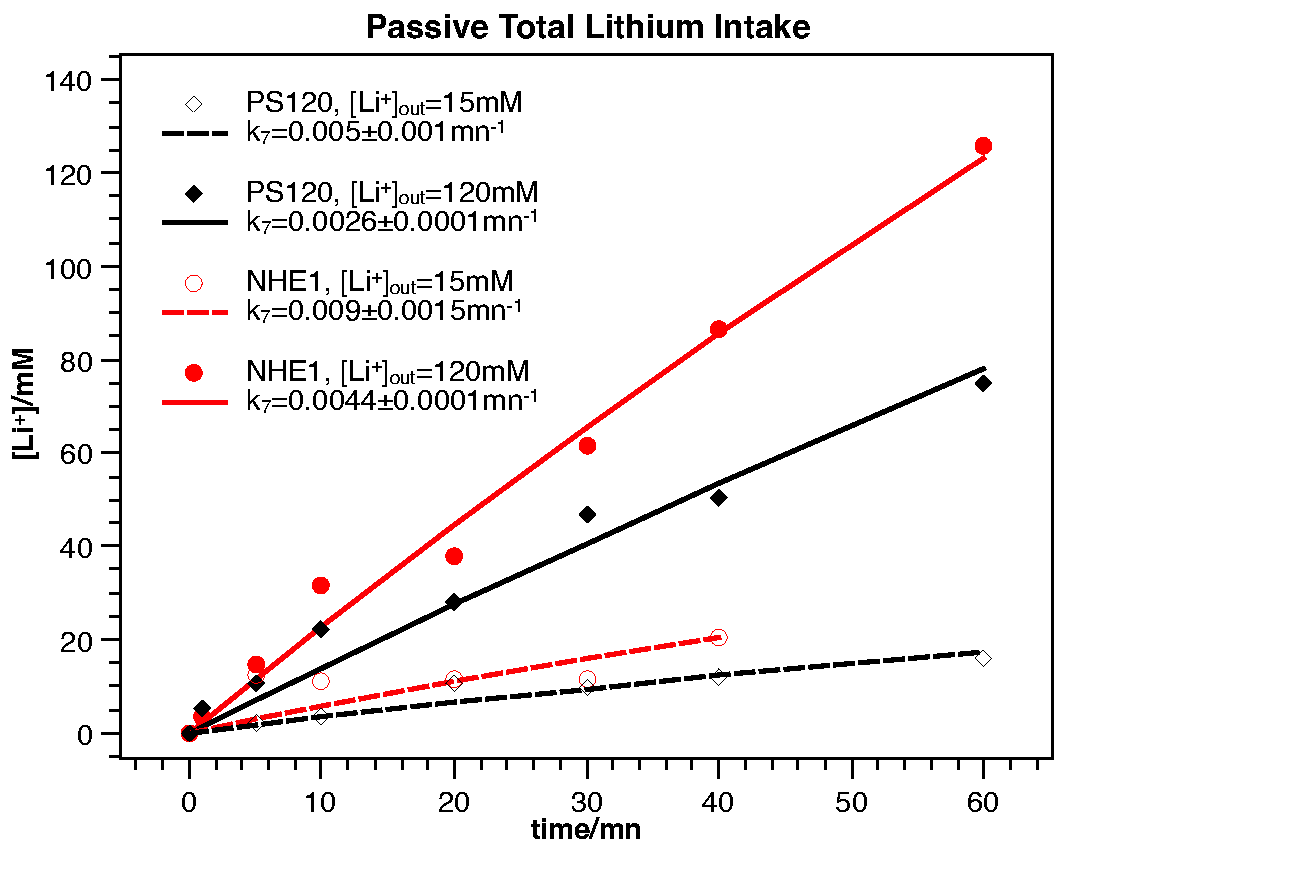
\includegraphics[width=0.5\textwidth]{leaks.pdf}
\end{center}
\caption{\label{fig:leak} Fit of experimental lithium electro-osmotic intake (points) according to the GHK theory (lines). Data were fitted with
Eq. \eqref{eq:LiAllKO} with $k_7$ as the variable.}
\end{figure}
For different lithium concentrations and cell types, we find some consistent leak constants.
Moreover, a set of isotopic sepatations for $\mychem{PS120}$ cells at $\LiAllOut=120\text{mM}$ were measured after 1 minute and it amounts to:
\begin{equation}
\label{eq:d7ps120}
\deltaLi^\ko_{@1\text{mn}} = 12.6435 \pm 0.025.
\end{equation}
If we assume that
for this case $k_7\approx0.0026\,\text{mn}^{-1}$, then
\begin{equation}
	\sigma^\ko \approx 1.0019 \pm 2\cdot10^{-5},
\end{equation}
which is a very good approximation \todo{given the crude assumptions} to the diffusive $\sigma=1.00229$. Accordingly, we will keep the more precise and documented $\sigma$ 
in the following theoretical and numerical work.

\subsection{Information from pH recovery}
Since the kinetic scheme depends on $\proton$, other measurements were performed to monitor the pH rise after the initial acidification, 
and are reported on Figure \ref{fig:protons} for different total external lithium concentrations. Since we do not include in this model the full homeostasis,
we take $\proton$ as an experiment-dependent input, and it appears that we get roughly:
\begin{equation}
\label{eq:hfit}
	\proton \simeq \proton_0 + \left(\proton_\infty-\proton_0\right) \dfrac{t}{t+t_h} = \proton_\infty + \left(\proton_0 - \proton_\infty\right) \dfrac{t_h}{t+t_h},
\end{equation}
and we use this equation to fit the current data as indicated on Figure \ref{fig:protons}. It is important to remember that $\proton_\infty$ depends on $\LiAllOut$.
From the measurements, we use an heuristic expression for $\proton$ dynamics depending on $\LiAllOut$:
\begin{equation}
\left\lbrace
\begin{array}{rcl}
t_h & = & \dfrac{A_h}{\erf\left(B_h\LiAllOut\right)}\\
A_h & = & 24.7      \pm 3.2 \text{ s}\\
B_h & = & 0.034     \pm 0.011\text{ mM}^{-1}\\ 
\end{array}
\right.
\end{equation}
and
\begin{equation}
\left\lbrace
\begin{array}{rcl}
\pH_0      & = & 5.92 \pm 0.2 \\
\pH_\infty & = & \pH_0 + \left(7.40-\pH_0\right) \dfrac{\LiAllOut}{\LiAll_h+\LiAllOut}\\
\LiAll_h   & = & 15.2\pm4.2\text{ mM}\\
\end{array}
\right.
\end{equation}


\begin{figure}[!ht]
\begin{center}
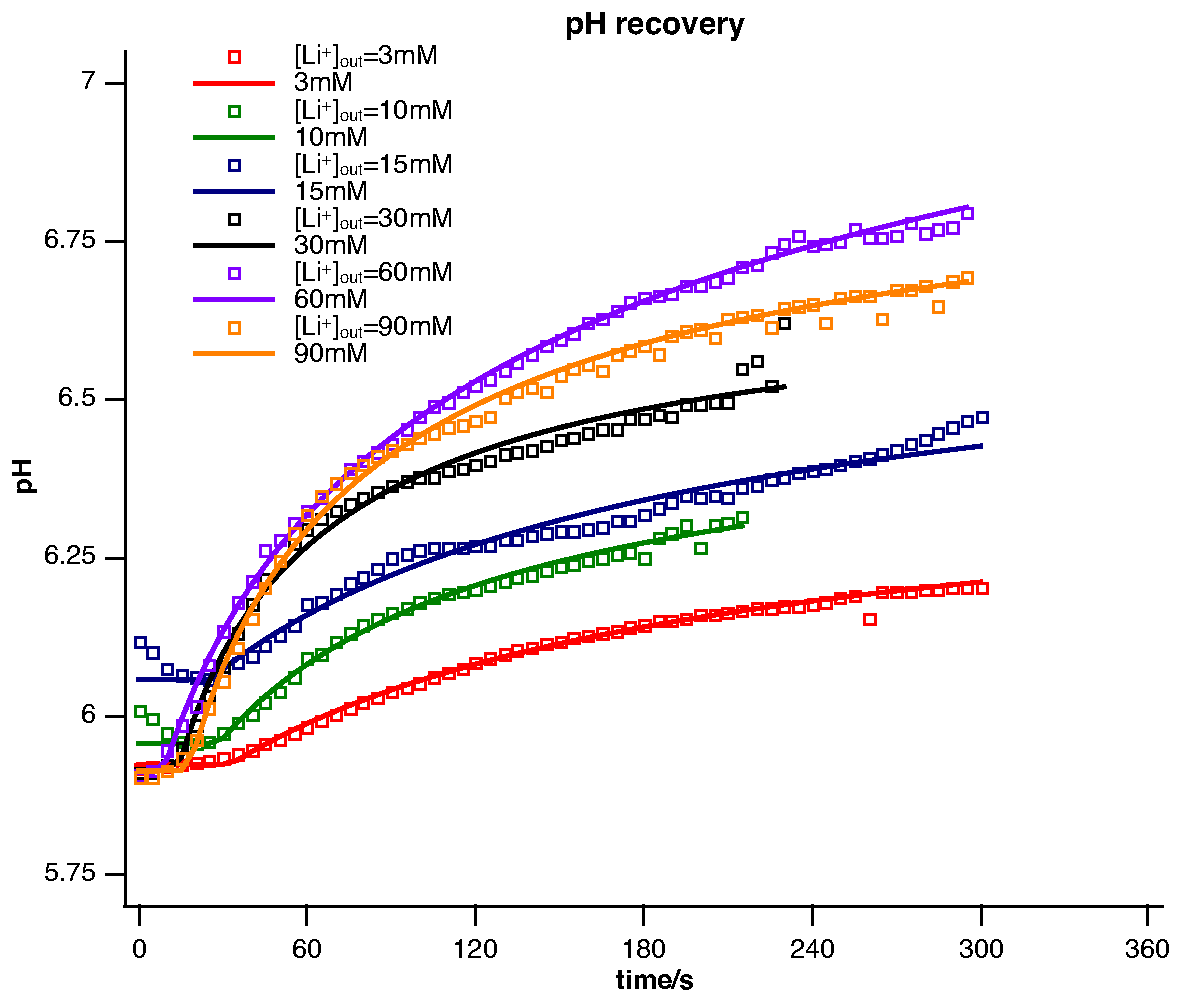
\includegraphics[width=0.5\textwidth]{protons.pdf}
\end{center}
\caption{\label{fig:protons} Fit (lines, according to Eq. \eqref{eq:hfit}) of apparent experimental protons intake (open circles).}
\end{figure}

\subsection{Information from another work about proton recycling}
The proton exit rate by $\NHE{1}$ was studied elsewhere \todo{ref EMBO Lacroix,Counillon}, and this rate depends itself on the inner pH.
From the data presented in figure 3a of that manuscript which shows that the $\NHE{1}$ turnover rate with $\proton$ is a sigmoid function, we
assume:
\begin{equation}
\label{eq:kh}
\left\lbrace
\begin{array}{rcl}
k_h & = & k_0 \eta(h)\\
\eta(h) & \approx & \dfrac{\left(\frac{h}{h_\eta}\right)^{p_\eta}}{1+\left(\frac{h}{h_\eta}\right)^{p_\eta}} \approx 
        \dfrac
{
10^{p_\eta(\mathrm{pH}_\eta-\mathrm{pH})}
}
{
1+10^{p_\eta(\mathrm{pH}_\eta-\mathrm{pH})}
}\\
h_\eta & = & 4\,10^{-7} \; \text{M}\\
\mathrm{pH}_\eta & = & 6.39 \\
p_\eta & = & 1.7 \\
\end{array}
\right.
\end{equation}
and we note that:
\begin{equation}
	\eta'(h) = \left(\dfrac{p_\eta}{h}\right) \dfrac{\left(\frac{h}{h_\eta}\right)^{p_\eta}}{\left[1+\left(\frac{h}{h_\eta}\right)^{p_\eta}\right]^2}  > 0
\end{equation}

\end{document}

\section{Linear System}
\subsection{System}
\begin{equation}
\label{eq:syslin}
\left\lbrace
\begin{array}{rcl}
\partial_t \hat\alpha & = &
	 k_h \left(1-\hat\alpha\right) 
	 - \LiAllOut    \hat\alpha\proton \Upsilon_\alpha  \\
	 \\
	\partial_t \beta_x & = & k_x\left(\Theta - \beta_x\right) +E_0  \hat\alpha  \proton \Upsilon_x \\
\end{array}
\right.
\end{equation}

	
\subsection{Initial Isotopic Separation}
We perform the short times integration of the system \eqref{eq:sysbis} using the initial
conditions \eqref{eq:ini} to get:
\begin{equation}
\beta_x(t) \underset{t\to0}{\approx} \left(k_x \Theta + E_0 \proton_0 \Upsilon_x\right) t,
\end{equation}
leading the initial ratio:
\begin{equation}
\label{eq:r0}
\left\lbrace
\begin{array}{rcl}
r_0 & = & \dfrac{k_7\Theta+E_0 \proton_0 \Upsilon_7}{k_6\Theta+E_0 \proton_0 \Upsilon_6}\\
	\\
    & = & \dfrac{k_7\Theta+E_0 \proton_0 \Upsilon_7}{ \sigma k_7\Theta+ \kappa E_0 \proton_0 \Upsilon_7}\\
\end{array}
\right.
\end{equation}
Accordingly, $r_0$ may vary between $\dfrac{1}{\sigma}$ and $\dfrac{1}{\kappa}$, so the only way for $\deltaLi$ to reach values
below $\deltaLi^\ko\simeq12.25$ is to satisfy $\kappa>\sigma$.

\subsection{Initial Active Speedup}
We measured the passive intake and the active intake (Laurent...)
and we found a speed up $s_0$ such that:
\begin{equation}
	\partial_t \Lambda_{\vert t\to0} \simeq s_0 \partial_t \Lambda^\ko_{\vert t\to0},
\end{equation}
leading to
\begin{equation}
\begin{array}{rcl}
	\partial_t \Lambda_{\vert t\to0} & = & \left[ (\epsilon_6 \sigma + \epsilon_7) k_7 \Theta + E_0 \proton_0 \Upsilon_\alpha \right] \LiAllOut \\
	& = & s_0 \left[  \underbrace{(\epsilon_6 \sigma + \epsilon_7)}_{\sigma'} k_7 \Theta \right] \LiAllOut,\\
\end{array}	
\end{equation}
so that
\begin{equation}
\label{eq:speedup}
	E_0 \proton_0 \Upsilon_\alpha = E_0 \proton_0 \kappa' \Upsilon_7 = (s_0-1)   \sigma' k_7 \Theta 
\end{equation}

\subsection{Final Isotopic Separation}
\begin{equation}
\label{eq:inf}
%\left\lbrace
\begin{array}{rcl}
	%\hat\alpha_\infty & = & \dfrac{k_0\eta(\proton_\infty)}{k_0\eta(\proton_\infty)+\LiAllOut \proton_\infty \Upsilon_\alpha}\\
	%\\
	\beta_x^\infty & = &\Theta + E_0 \hat\alpha_\infty \proton_\infty \dfrac{\Upsilon_x}{k_x}\\
\end{array}
%\right.
\end{equation}


\subsection{Parameters evaluation}
From \eqref{eq:speedup}, we gain the expression of the \underline{catalytic ratio} $\mu$ by:
\begin{equation}
\label{eq:mu_def}
	\dfrac{\proton_0 E_0 \Upsilon_7}{k_7} = \Theta \underbrace{\left(s_0-1\right) 
	\dfrac{ \sigma' }{\kappa'}}_{\mu},
\end{equation}
leading to
\begin{equation}
	\mu = \dfrac{ r_0 \sigma' \left(s_0-1\right) - \epsilon_6\left(1-r_0\sigma\right)}{\epsilon_7 r_0 + \epsilon_6 }
\end{equation}

We inject this expression into to get the ratios:
\begin{equation}
\left\lbrace
\begin{array}{rcl}
	r_0 & = & \dfrac{1+\mu}{\sigma+\kappa\mu}\\
	\\
	\varphi & = &   \dfrac{\hat\alpha \proton}{\proton_0}\\
	\\
	\gamma_h & = &  \dfrac{\proton_\infty}{\proton_0} \;\; \left(\Rightarrow \varphi_\infty = \gamma_h \hat\alpha_\infty\right)\\
	\\
	r_\infty & = &
	 \dfrac{\Theta + E_0 \hat\alpha_\infty \proton_\infty \dfrac{\Upsilon_7}{k_7} }
	 {\Theta + E_0 \hat\alpha_\infty \proton_\infty \dfrac{\Upsilon_6}{k_6}}
	 =\dfrac{1 + \varphi_\infty \mu }{1+ \varphi_\infty \dfrac{\kappa}{\sigma}\mu}
\end{array}
\right.
\end{equation}

From the experiments we estimate:
\begin{equation}
\dfrac{1}{r_0}  >  \sigma,
\end{equation}
so that we choose:
\begin{equation}
\mu > 0,
\end{equation}
to get the matching expression for $\kappa$:
\begin{equation}
\left\lbrace
\begin{array}{rcl}
	\kappa  & = &  \dfrac{1+\mu}{\mu}\left[\dfrac{1}{r_0} - \dfrac{\sigma}{1+\mu}\right] 
	=  \sigma + {\dfrac{1+\mu}{\mu}\left[ \dfrac{1}{r_0} - \sigma \right]} \; (\kappa>\sigma)\\
	\\
	\dfrac{\kappa}{\sigma} & = & 1 + {\dfrac{1+\mu}{\mu}\left[ \dfrac{1}{r_0\sigma} - 1\right]} \; \left(\dfrac{\kappa}{\sigma}> 1\right)\\
	\\
	\mu \dfrac{\kappa}{\sigma} & = & \dfrac{1+\mu}{r_0\sigma} - 1 = \mu'\\
	\\
 \kappa & > & \dfrac{1}{r_0} > \sigma \;\Rightarrow\; \dfrac{\sigma}{\kappa} < \sigma r_0  < 1\\
\end{array}
\right.
\end{equation}
These expressions arising from the initial conditions are directly influencing the steady state values:
\begin{equation}
\label{eq:r_ss}
\left\lbrace
\begin{array}{rcl}
	r_\infty & = & \dfrac{1+\mu \varphi_\infty}{1+\left(\dfrac{1+\mu}{r_0\sigma} - 1\right)\varphi_\infty} \geq r_0 \sigma\\
	\\
	& = & \dfrac{1+\mu \gamma_h \hat\alpha_\infty}{1+\mu'\gamma_h \hat\alpha_\infty} 
\end{array}
\right.
\end{equation}
We show that to recover a high $r_\infty$, we must have $\varphi_\infty\leq 1$, and \textbf{we will assume that $\gamma_h\leq1$}.
For any $\mu$:
\begin{equation}
	r_0\sigma \leq \dfrac{1+\mu\gamma_h}{1+\mu' \gamma_h} < r_\infty < 1.
\end{equation}
We define:
\begin{equation}
	r_\mu = \dfrac{1+\mu\gamma_h}{1+\mu' \gamma_h}
\end{equation}
and we get the value
\begin{equation}
\left\lbrace
\begin{array}{rcl}
	\hat\alpha_\infty & = & \dfrac{\left(1-r_\infty\right)}
	{ \left(1-r_\infty\right) + 
	\left[1+\mu' \gamma_h\right] \left(r_\infty-r_\mu\right)
	} \\
	\\
	& = & \cos^2 \Omega\\
	\\
	& = & \dfrac{k_0\eta_\infty}{k_0\eta_\infty+\LiAllOut \proton_\infty \Upsilon_\alpha}\\
	\\
	& = & \dfrac{1}{1+\dfrac{\LiAllOut \proton_\infty \Upsilon_\alpha}{k_0\eta_\infty}}\\
\end{array}
\right.
\end{equation}
This means that one $\hat\alpha_\infty = \cos^2 \Omega $ is computed, this imposes the scaling:
\begin{equation}
	\LiAllOut \Upsilon_\alpha \proton_\infty = {k_0\eta_\infty} \tan^2\Omega,\;\;  \tan^2\Omega = \dfrac{1-\hat\alpha_\infty}{\hat\alpha_\infty}
\end{equation}


\begin{equation}
\left\lbrace
\begin{array}{rcl}
	 \varphi(t) & = & \dfrac{\hat\alpha(t) \proton}{\proton_0}\\
	 \\
	  \partial_t \hat\alpha & = &
	 k_0  \left[ \eta\left(\proton\right) \left(1-\hat\alpha\right) 
	 -  \dfrac{\eta_\infty}{\proton_\infty} \proton \hat\alpha \tan^2\Omega\right]   \\
	 \\
	 & = &
	 k_0 \eta_0 \left[ \dfrac{\eta( \proton )}{\eta_0} \left(1-\hat\alpha\right) 
	 - \dfrac{\eta_\infty}{\eta_0} \dfrac{\proton_0}{\proton_\infty} \varphi(t) \tan^2\Omega\right]   \\
	 \\
	\partial_t \beta_7 & = & k_7 \left[ \Theta \left( 1 + \mu \varphi(t) \right) - \beta_7 \right] \\
	\\
	\partial_t \beta_6 & = & \sigma k_7 \left[ \Theta \left( 1 + \mu' \varphi(t) \right) -  \beta_6 \right] \\
\end{array}
\right.
\end{equation}

\subsection{Short Times integration}
\begin{equation}
\left\lbrace
\begin{array}{rcl}
	\partial_t \hat\alpha & = & k_0 \left[ \dfrac{\eta(\proton)}{\eta_0} - \left[ \omega^2 \dfrac{\proton}{\proton_0} + \dfrac{\eta(\proton)}{\eta_0} \right] \hat\alpha \right], \;\; \omega^2 = \dfrac{\eta_\infty}{\eta_0}\dfrac{\proton_0}{\proton_\infty}\tan^2\Omega\\
	\\
	\rho(u) & = & \dfrac{\proton}{\proton_0}\\
	\dfrac{\eta(\proton)}{\eta_0} & \simeq & \rho( v_0 t)  \\
	v_0 & = & \dfrac{p_\eta}{1+\left(\frac{\proton_0}{h_\eta}\right)^{p_\eta}}\simeq 0.233\text{ for $\pH_0=5.92$, does not depend on $t_h$}\\
	\\
\partial_t\hat\alpha	 & \simeq &  f(v_0t) - \left[ \omega^2 f(t) +  f(v_0t) \right] \hat\alpha,\;\;f(t) = k_0 \rho(t) \\
	 F(t) & = & \int_0^t f(u) \; \mathrm{d}u \\
	 \tilde F(t) & = & \int_0^t f(v_0 u) \; \mathrm{d}u = \dfrac{1}{v_0} F(v_0t)\\
\end{array}
\right.
\end{equation}

\begin{equation}
		 \hat\alpha(t) =  \left[ 1 + \int_0^t f(v_0u) e^{\left[\omega^2 F(u)+\frac{1}{v_0}F(v_0u)\right]}\;\mathrm{d}u\right]
		  e^{-\left[\omega^2 F(t)+\frac{1}{v_0}F(v_0 t)\right]}
\end{equation}

\begin{equation}
	f(t) = k_0\left[ 1 - \delta_h \dfrac{t}{t+t_h} \right] = k_0\left[ 1 - \delta_h \left( 1- \dfrac{t_h}{t+t_h}\right) \right] 
	= k_0 \left[ (1-\delta_h) + \delta_h \dfrac{t_h}{t+t_h}\right]
\end{equation}

\begin{equation}
\left\lbrace
\begin{array}{rcl}
 F(t) & = & k_0 \left[ (1-\delta_h) t + \delta_h t_h \ln\left( 1+ \dfrac{t}{t_h}\right)\right]\\
 \\
 \dfrac{1}{v_0}F(v_0t) & = & k_0 \left[ (1-\delta_h) t + \delta_h \dfrac{t_h}{v_0} \ln\left( 1+ \dfrac{tv_0}{t_h}\right)\right] \\
\end{array}
\right.
\end{equation}

For $t\ll t_h$,
\begin{equation}
\left\lbrace
\begin{array}{rcl}
	f(t) & \simeq & k_0 \left[1-\delta_h \dfrac{t}{t_h}\right]\\
	\\
	f(v_0u) & \simeq & 	k_0 \left[1-\delta_h \dfrac{v_0u}{t_h}\right]\\
	\\
	F(t) & \simeq & k_0 t \left[1 - \dfrac{\delta_h}{2}\dfrac{t}{t_h}\right]\\
	\\
	\dfrac{1}{v_0} F(v_0t) & \simeq & k_0 t \left[ 1 - \dfrac{\delta_h}{2}\dfrac{v_0t}{t_h}\right] \\
	\\
	\omega^2 F(t) + \dfrac{1}{v_0} F(v_0t)& \simeq & k_0 t \left[ (1+\omega^2) - \dfrac{\delta_h\left(\omega^2+v_0\right)}{2} \dfrac{t}{t_h}\right]\\
\end{array}
\right.
\end{equation}

\begin{equation}
\left\lbrace
\begin{array}{rcl}
	\partial_t \beta_x  & = & k_x \left[ \Theta\left( 1 + \mu_x \rho(t) \hat\alpha(t) \right)- \beta_x\right]\\
	\\
	\beta_x(t) & = & \displaystyle k_x\left[ \int_0^t \left[ \Theta\left( 1 + \mu_x \rho(u) \hat\alpha(u) \right) \right] e^{k_xu} \; \mathrm{d} u \right] e^{-k_x t}\\
\end{array}
\right.
\end{equation}


\end{document}

\section{Passive Return}
Let us assume that for a given time $t^\start$ we get the values $\beta_x^\start$ such that $\beta_6^\start+\beta_7^\start=B^\start\Theta$ and a given isotopic ratio $r^\start$:
\begin{equation}
\label{eq:start}
\left\lbrace
\begin{array}{rcl}
\beta_6^\start+\beta_7^\start & = & B^\start\Theta \\
\\
\dfrac{\beta_7^\start}{\beta_6^\start} & = & r^\start\\
\end{array}
\right.
\Rightarrow
\left\lbrace
\begin{array}{rcl}
\beta_7^\start & = & \dfrac{r^\start B^\start}{1+r^\start}\Theta\\
\\
\beta_6^\start & = & \dfrac{B^\start}{1+r^\start}\Theta\\
\\
\beta_x(t\geq t^\start) & = & \beta_x^\start + \left(\Theta-\beta_x^\start\right)\left[1-e^{-k_x(t-t^\start)}\right]\\
\end{array}
\right.
\end{equation}
which defines the relaxing separation ratio:
\begin{equation}
	r(t\geq t^\start) = \dfrac
	{
		r^\start B^\start + ( 1+r^\start - r^\start B^\start) \left[1-e^{-k_7(t-t^\start)}\right]
	}
	{
		 B^\start + ( 1+r^\start -  B^\start) \left[1-e^{-k_7\sigma(t-t^\start)}\right]
	}
\end{equation}





\end{document}
